Porous materials have the capability of absorbing moisture from an environment of air due to adsorption forces, 
attracting molecules of vapor to the solid parts of the porous system, and due to the depression of water pressure 
because of the tension over the concave menisci of the water filled capillaries. Moisture in materials can be therefore 
present as moist air, water and ice or in some intermediate state 
as adsorbed phase on the pore walls, respectively. Since it is in general not possible to distinguish the different 
aggregate states, the water content is defined as the ratio of the total moisture weight to the dry weight 
of the material \cite{ctu}. Equilibrium of the water content with its local environment is represented by a retention curve 
of the material, relating the moisture and the relative humidity $h$ of the surrounding air. 

The {\it moisture retention curve} is composed of three parts Fig.~(\ref{reten}): 
the {\it sorption isotherm} up to about 95 \% 
- 98 \% relative humidity $RH$ (region I), the capillary moisture (region II), and the over-saturated region III, where 
the water retention function is a vertical line at 100 \% $RH$. As is demonstrated in Fig.~\ref{reten}, a higher 
temperature level results in lower moisture content for the same relative humidity. In the region II it is difficult 
to determine $w$ unambiguously by sorption tests. However, there still exists equilibrium between two porous materials 
up to the capillary saturation with a suction stress close to zero (a material is in contact with liquid water). 
In order to fill all pores, a high pressure or vacuum has to be applied in the region III. In this region, 
no well-defined function exists between the water content and the relative humidity or the suction stress, respectively, 
and therefore, no well-defined moisture equilibrium between two porous material samples might be expected.
\begin{figure}[h!]
\begin{center}
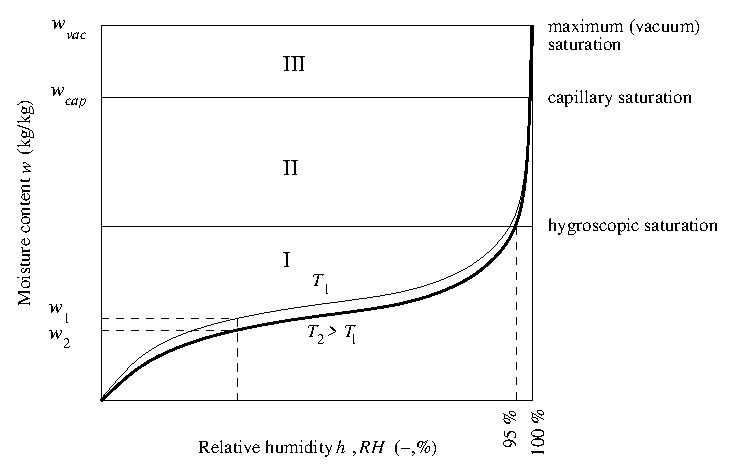
\includegraphics[angle=0, width=10cm]{PS/reten.eps}
\caption{Sorption isotherms}
\label{reten}
\end{center}
\end{figure}

In the transient region II, there is a relationship between the relative humidity, the water content (saturation) 
and the capillary pressure in the pores \cite{lewis}
\begin{eqnarray}\label{cap_press}
p^c = p^g - p^w,
\end{eqnarray}
where $p^w > 0$ is the pressure of the liquid phase (water). 

\subsubsection{Pedersen model}

\begin{center}
\begin{tabular}{|l|l|}
\hline
location & /TRFEL/SRC/bazped.cpp\\
         & /TRFEL/SRC/bazped.h\\
         & /TRFEL/SRC/pedersen.cpp\\
         & /TRFEL/SRC/pedersen.h
\\ \hline
related files &
\\ \hline
notes & 
\\ \hline
\end{tabular}
\end{center}

The sorption isotherm is approximated by this simple formula \cite{pedersen}
\begin{eqnarray}\label{sorption_isotherm}
w = w_h \Big(1 - \frac{\ln h}{A}\Big)^{-\frac{1}{n}},
\end{eqnarray}
where $h$ is relative humidity and $w_h$, $A$, $n$ are material parameters.

An analytical expression is proposed for the saturation vapor pressure as a function of temperature $T[{\rm K}]$ 
\begin{eqnarray}\label{saturation_pressure}
p^{gws}(T) = \exp \Big(23,5771 - \frac{4042,9}{T-37,58}\Big) \quad ({\rm Pa}).
\end{eqnarray}

\subsubsection{JM model}
\begin{center}
\begin{tabular}{|l|l|}
\hline
location & /TRFEL/SRC/kunzel.cpp\\
         & /TRFEL/SRC/kunzel.h
\\ \hline
related files &
\\ \hline
notes & 
\\ \hline
\end{tabular}
\end{center}
